\documentclass{article}
\usepackage{ctex}
\usepackage{graphics}
\usepackage{geometry}
\usepackage{listings}
% bmeps -c test.png test.eps
\geometry{left=2.0cm,right=2.0cm,top=2.0cm,bottom=2.0cm}
\title{NoSQL数据库}
\author{pwlin1992@gmail.com}
\begin{document}
\maketitle
\tableofcontents
\begin{large}
  \section{NoSQL简介}
  \paragraph{灵活的可扩展性}\mbox{} \\
  RDBMS很难实现“横向扩展”,在面对数据库负载大规模增加时,往往需要通过\textcolor{red}{\textbf{升级硬件}}来实现“纵向扩展”。

  横向扩展:一个DBMS不够用,则用两个,三个。

  纵向扩展:一个DBMS不够用,则升级硬件,使其更快。

  NoSQL在设计之初就是为了满足“横向扩展”的需求,因此天生具备良好的水平扩展能力。
  \paragraph{灵活的数据模型}\mbox{} \\
  摆脱RDBMS的各种束缚条件,采用键/值、列族等非关系模型,允许在一个数据元素里存储不同类型的数据。

  \paragraph{与云计算紧密融合}\mbox{} \\
  云计算具有很好的水平扩展能力,可以根据资源使用情况进行自由伸缩,各种资源可以动态加入或退出。NoSQL数据库可以凭借自身良好的横向扩展能力,充分自由利用云计算基础设施,很好地融入到云计算环境中,构建基于NoSQL的云数据库服务。

  \section{NoSQL兴起的原因}
  \subsection{RDBMS无法满足Web 2.0的需求}
  \paragraph{无法满足海量数据的管理需求}\mbox{} \\
  对于RDBMS来说,在一张10亿条记录的表里进行SQL查询,效率极其低下。

  \paragraph{无法满足数据高并发的需求}\mbox{} \\
  在Web 1.0时代,通常采用动态页面静态化技术,事先访问数据库生成静态页面供浏览者访问,从而保证在大规模用户访问时,也能够获得较好的实时响应性能。但是在Web 2.0时代,各种用户都在不断地发生更新,如:购物记录、搜索记录等信息都需要实时更新,动态页面静态化技术基本无用武之地,所有信息都需要动态实时生成,这就会导致高并发的数据库访问,可能产生每秒上万次的读写请求,对于很多RDBMS而言都是难以承受的。

  \paragraph{无法满足高可扩展性和高可用性的需求}\mbox{} \\
  在Web 2.0时代,不知名的网站可能一夜爆红,知名网站也有可能因为发布了热门信息而引来大量用户围观,这些都会导致对数据库读写负荷的急剧增加,需要数据库能够在短时间内迅速提升性能应对突发需求。而RDBMS难以水平扩展,无法像网页服务器和应用服务器那样简单通过添加更多硬件和服务节点来扩展性能和负载能力。

  \subsection{NoSQL与RDBMS的对比}
  \begin{figure}[htbp]
    \centering
    \caption{NoSQL与RDBMS的对比}
    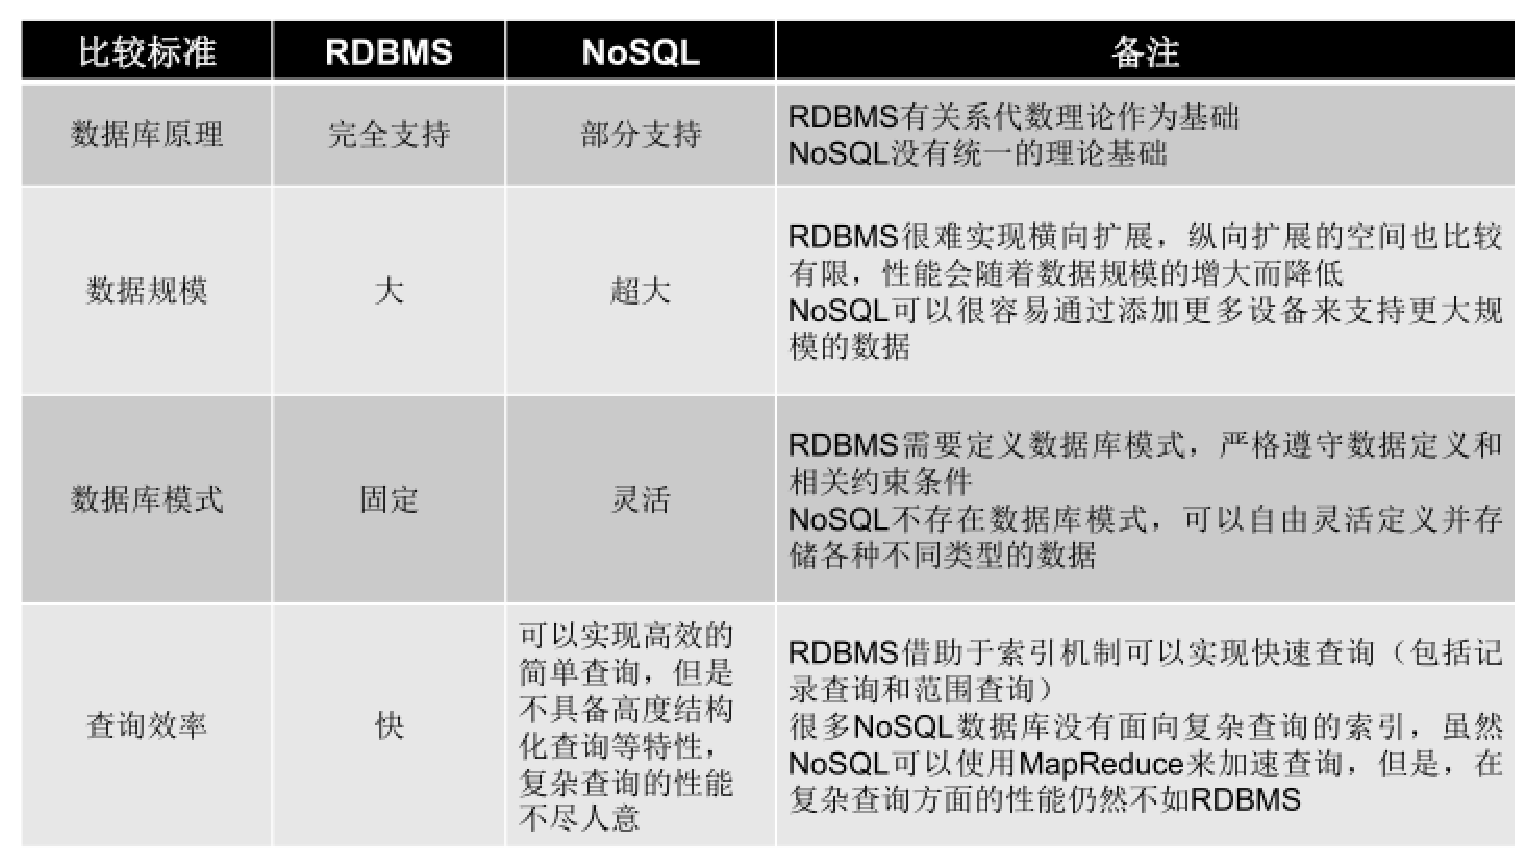
\includegraphics[scale=0.5]{0.eps}
    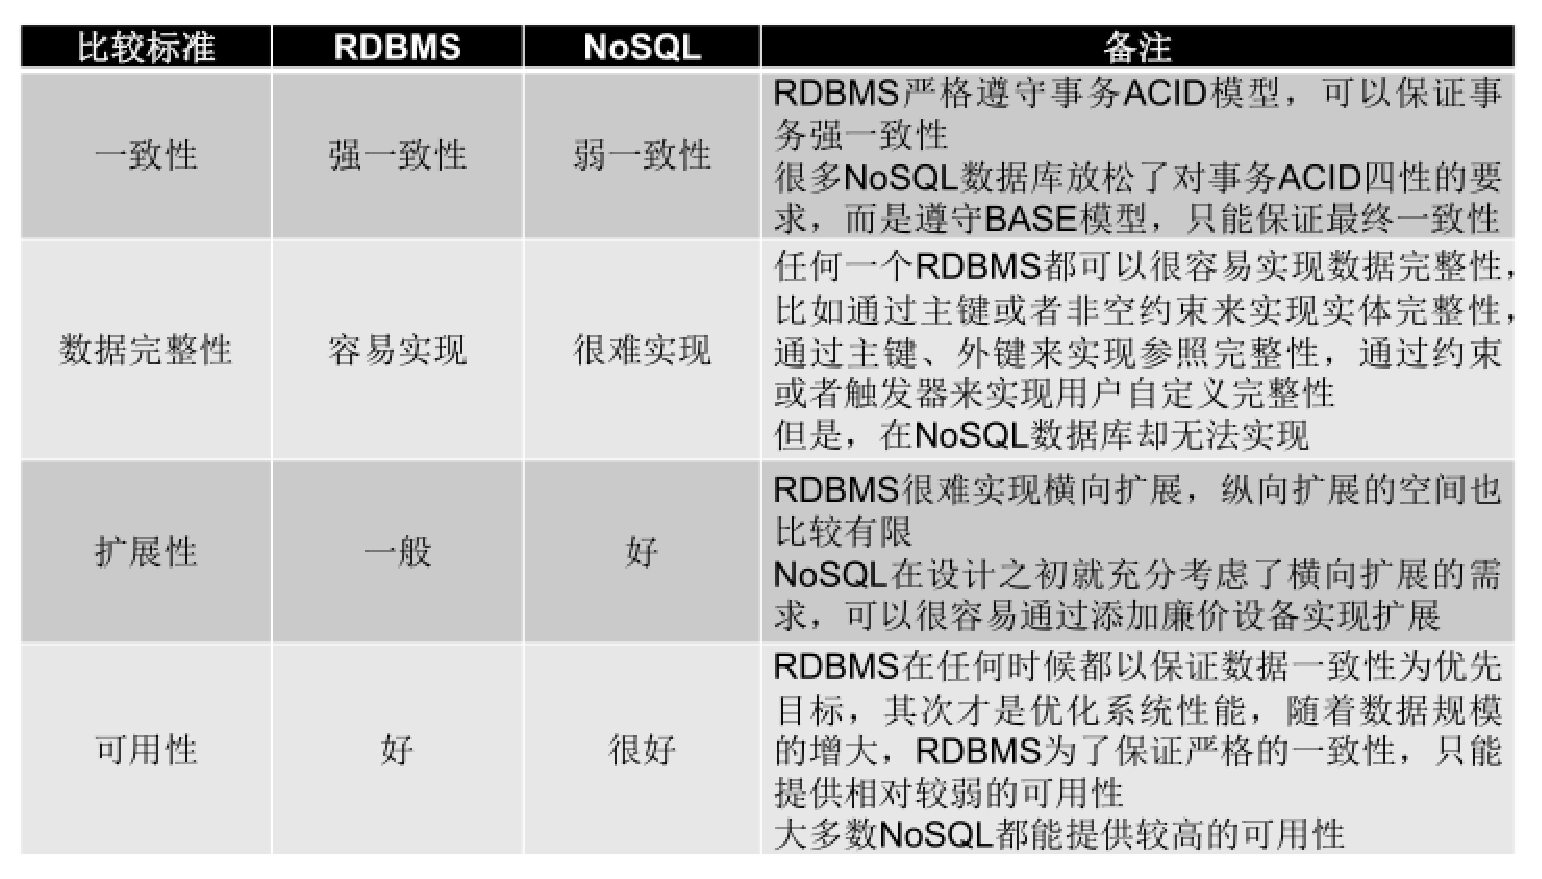
\includegraphics[scale=0.5]{1.eps}
    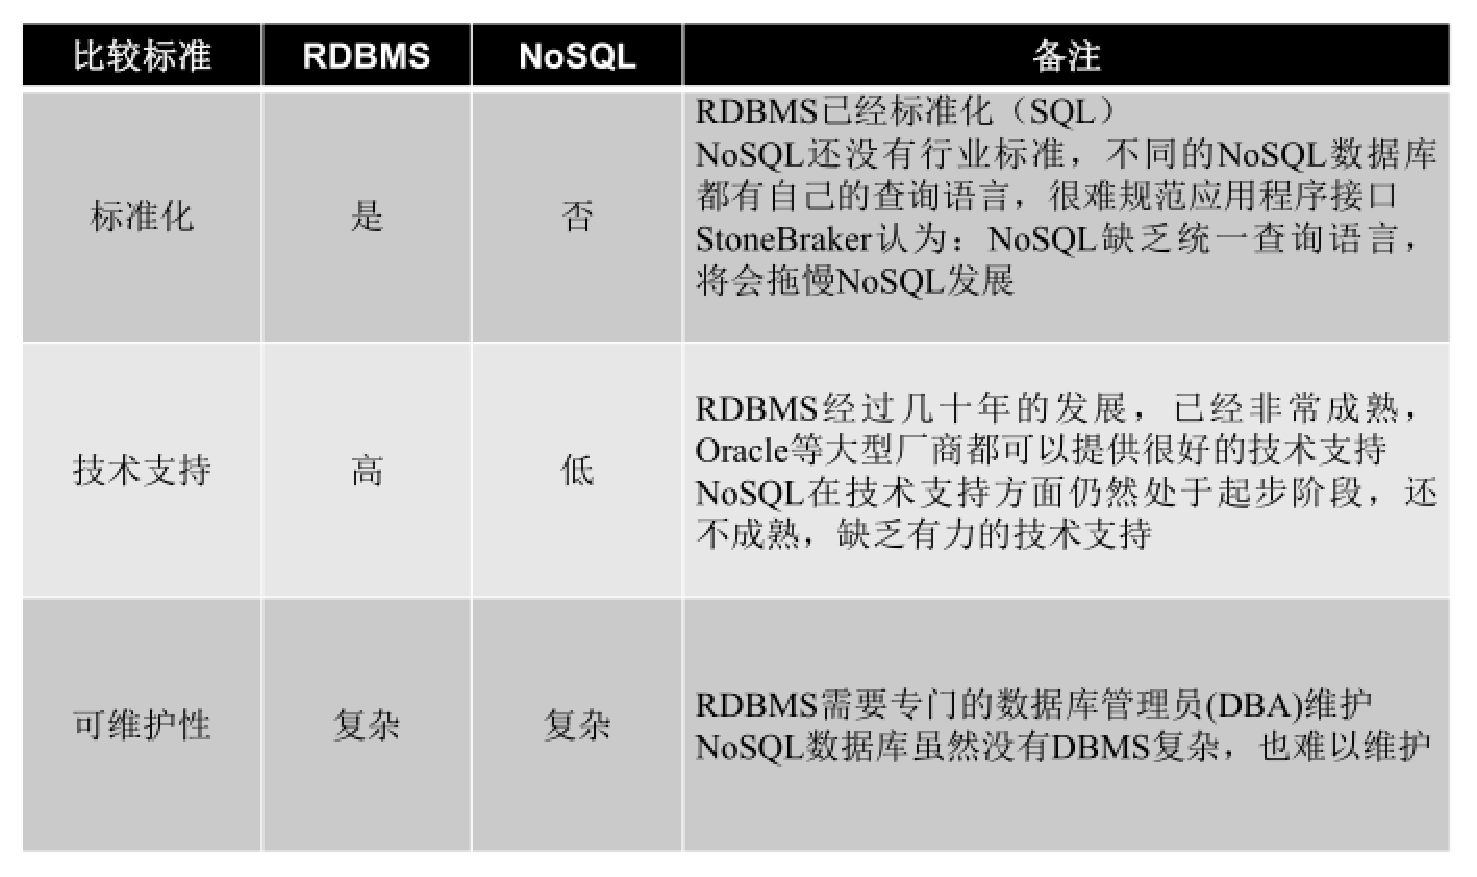
\includegraphics[scale=0.5]{2.eps}
  \end{figure}
  NoSQL与RDBMS各有优劣,NoSQL缺乏数学理论基础,复杂查询性能不高,不能实现事务强一致性,很难实现数据完整性。在实际应用中,公司一般会采用两者混合使用的方式,如:对于购物车这种临时性数据,采用键值存储会更加高效,而当前产品和订单信息则适合存放在关系数据库中,大量的历史订单信息则适合保存在类似MongoDB的文档数据库中。

  \section{NoSQL的类型}
  \subsection{键值数据库}
  \begin{figure}[h]
    \centering
    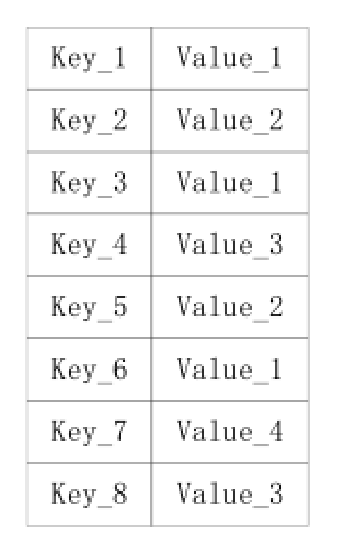
\includegraphics{3.eps}
    \caption{键值数据库}
  \end{figure}
  键值数据库使用哈希表,表中的key可以用来定位value,即存储和检索具体的value。value对数据库而言是不可见的,不能对value进行索引和查询,只能通过key进行查询,value可以存储任意类型的数据。

  在存在大量写操作的情况下,键值数据库可以比关系数据库取得明显更好的性能。因为RDBMS需要建立索引来加速查询,当存在大量写操作时,索引会发生频繁更新,由此会产生高昂的索引维护代价。

  \begin{figure}[h]
    \centering
    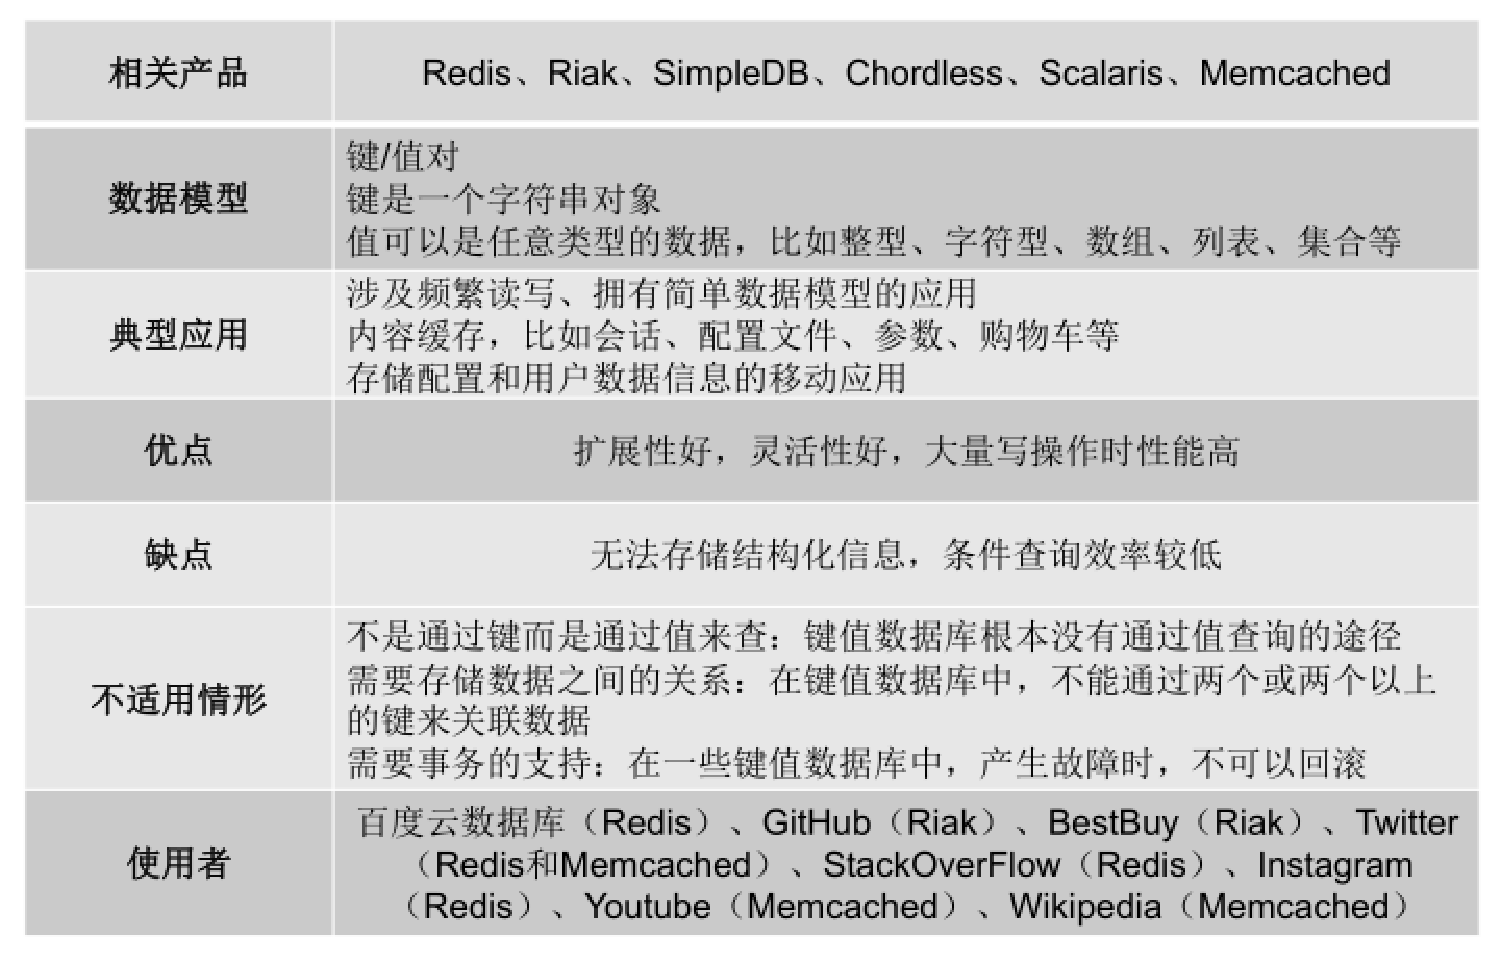
\includegraphics[scale=0.5]{4.eps}
    \caption{键值数据库}
  \end{figure}

  \subsection{列族数据库}
\end{large}
\end{document}

%%% Local Variables:
%%% mode: latex
%%% TeX-master: t
%%% End:
